%\documentclass{standalone}
%\usepackage{tikz}
%\usetikzlibrary{patterns,plotmarks}
%\begin{document}
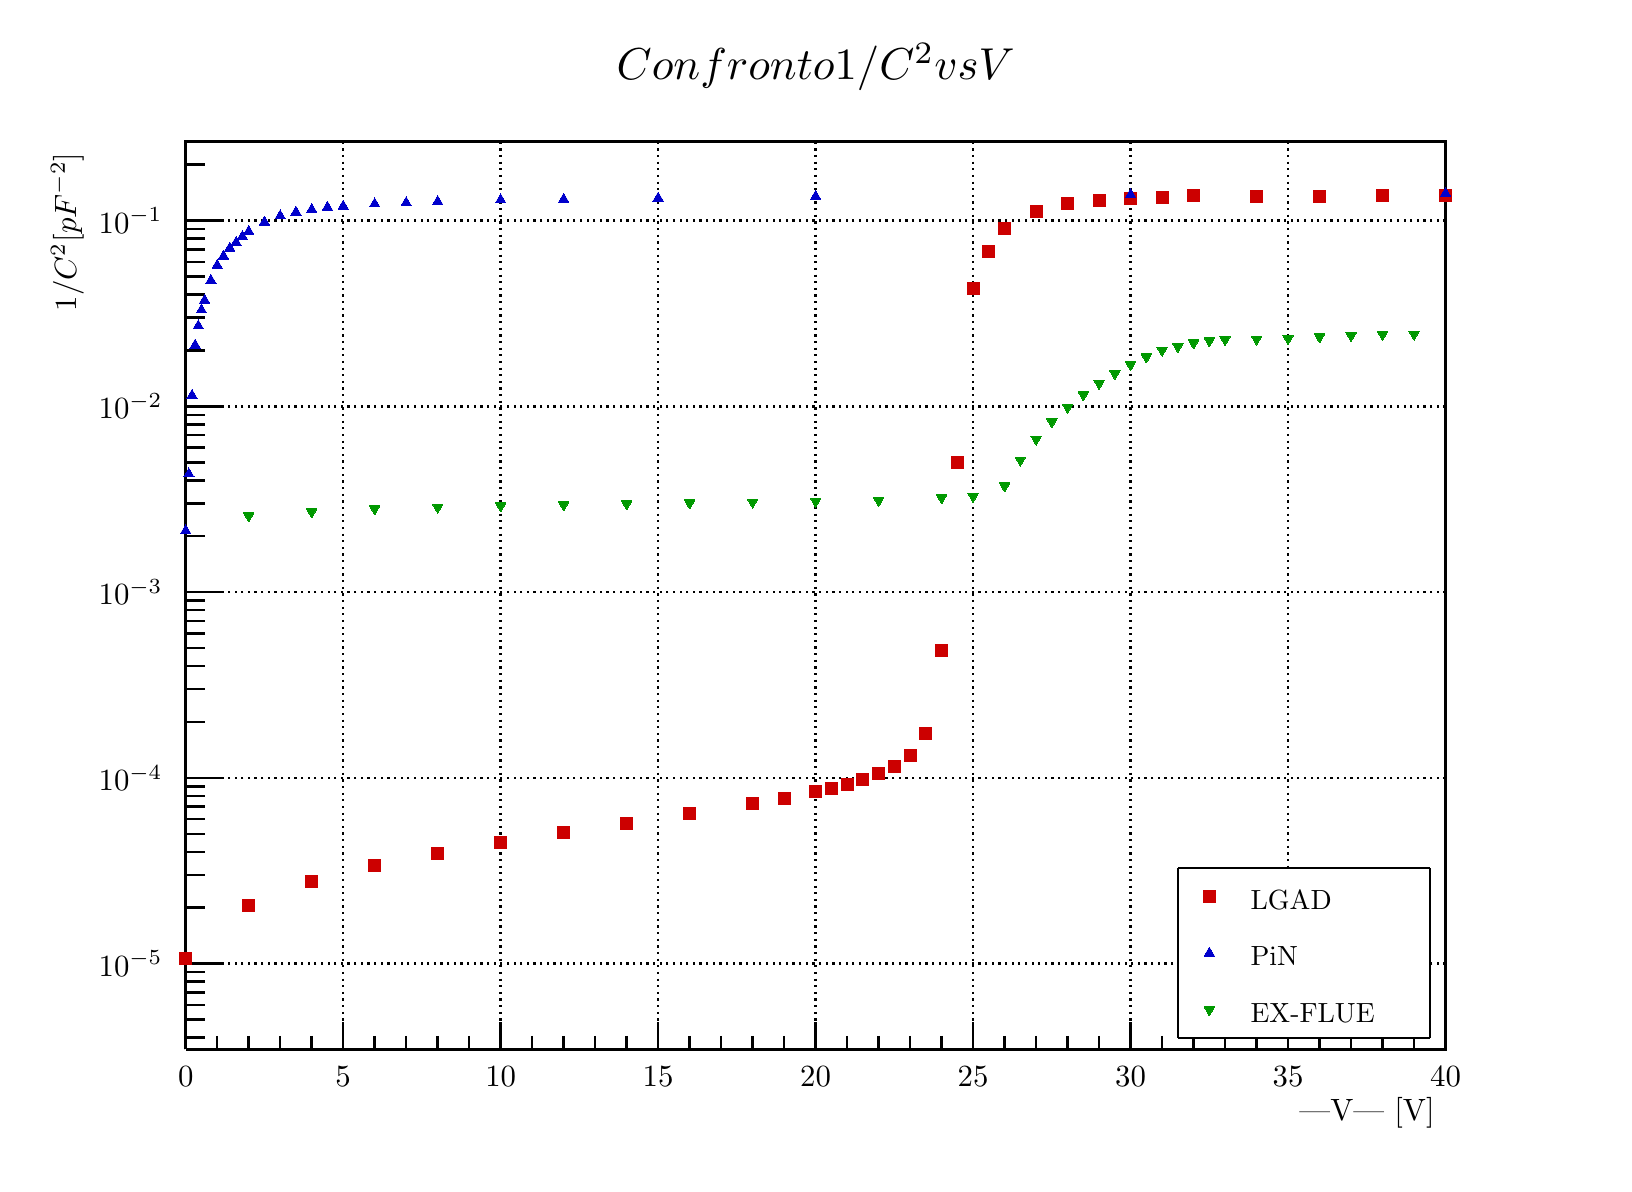
\begin{tikzpicture}
\def\CheckTikzLibraryLoaded#1{ \ifcsname tikz@library@#1@loaded\endcsname \else \PackageWarning{tikz}{usetikzlibrary{#1} is missing in the preamble.} \fi }
\CheckTikzLibraryLoaded{patterns}
\CheckTikzLibraryLoaded{plotmarks}
\pgfdeclareplotmark{cross} {
\pgfpathmoveto{\pgfpoint{-0.3\pgfplotmarksize}{\pgfplotmarksize}}
\pgfpathlineto{\pgfpoint{+0.3\pgfplotmarksize}{\pgfplotmarksize}}
\pgfpathlineto{\pgfpoint{+0.3\pgfplotmarksize}{0.3\pgfplotmarksize}}
\pgfpathlineto{\pgfpoint{+1\pgfplotmarksize}{0.3\pgfplotmarksize}}
\pgfpathlineto{\pgfpoint{+1\pgfplotmarksize}{-0.3\pgfplotmarksize}}
\pgfpathlineto{\pgfpoint{+0.3\pgfplotmarksize}{-0.3\pgfplotmarksize}}
\pgfpathlineto{\pgfpoint{+0.3\pgfplotmarksize}{-1.\pgfplotmarksize}}
\pgfpathlineto{\pgfpoint{-0.3\pgfplotmarksize}{-1.\pgfplotmarksize}}
\pgfpathlineto{\pgfpoint{-0.3\pgfplotmarksize}{-0.3\pgfplotmarksize}}
\pgfpathlineto{\pgfpoint{-1.\pgfplotmarksize}{-0.3\pgfplotmarksize}}
\pgfpathlineto{\pgfpoint{-1.\pgfplotmarksize}{0.3\pgfplotmarksize}}
\pgfpathlineto{\pgfpoint{-0.3\pgfplotmarksize}{0.3\pgfplotmarksize}}
\pgfpathclose
\pgfusepathqstroke
}
\pgfdeclareplotmark{cross*} {
\pgfpathmoveto{\pgfpoint{-0.3\pgfplotmarksize}{\pgfplotmarksize}}
\pgfpathlineto{\pgfpoint{+0.3\pgfplotmarksize}{\pgfplotmarksize}}
\pgfpathlineto{\pgfpoint{+0.3\pgfplotmarksize}{0.3\pgfplotmarksize}}
\pgfpathlineto{\pgfpoint{+1\pgfplotmarksize}{0.3\pgfplotmarksize}}
\pgfpathlineto{\pgfpoint{+1\pgfplotmarksize}{-0.3\pgfplotmarksize}}
\pgfpathlineto{\pgfpoint{+0.3\pgfplotmarksize}{-0.3\pgfplotmarksize}}
\pgfpathlineto{\pgfpoint{+0.3\pgfplotmarksize}{-1.\pgfplotmarksize}}
\pgfpathlineto{\pgfpoint{-0.3\pgfplotmarksize}{-1.\pgfplotmarksize}}
\pgfpathlineto{\pgfpoint{-0.3\pgfplotmarksize}{-0.3\pgfplotmarksize}}
\pgfpathlineto{\pgfpoint{-1.\pgfplotmarksize}{-0.3\pgfplotmarksize}}
\pgfpathlineto{\pgfpoint{-1.\pgfplotmarksize}{0.3\pgfplotmarksize}}
\pgfpathlineto{\pgfpoint{-0.3\pgfplotmarksize}{0.3\pgfplotmarksize}}
\pgfpathclose
\pgfusepathqfillstroke
}
\pgfdeclareplotmark{newstar} {
\pgfpathmoveto{\pgfqpoint{0pt}{\pgfplotmarksize}}
\pgfpathlineto{\pgfqpointpolar{44}{0.5\pgfplotmarksize}}
\pgfpathlineto{\pgfqpointpolar{18}{\pgfplotmarksize}}
\pgfpathlineto{\pgfqpointpolar{-20}{0.5\pgfplotmarksize}}
\pgfpathlineto{\pgfqpointpolar{-54}{\pgfplotmarksize}}
\pgfpathlineto{\pgfqpointpolar{-90}{0.5\pgfplotmarksize}}
\pgfpathlineto{\pgfqpointpolar{234}{\pgfplotmarksize}}
\pgfpathlineto{\pgfqpointpolar{198}{0.5\pgfplotmarksize}}
\pgfpathlineto{\pgfqpointpolar{162}{\pgfplotmarksize}}
\pgfpathlineto{\pgfqpointpolar{134}{0.5\pgfplotmarksize}}
\pgfpathclose
\pgfusepathqstroke
}
\pgfdeclareplotmark{newstar*} {
\pgfpathmoveto{\pgfqpoint{0pt}{\pgfplotmarksize}}
\pgfpathlineto{\pgfqpointpolar{44}{0.5\pgfplotmarksize}}
\pgfpathlineto{\pgfqpointpolar{18}{\pgfplotmarksize}}
\pgfpathlineto{\pgfqpointpolar{-20}{0.5\pgfplotmarksize}}
\pgfpathlineto{\pgfqpointpolar{-54}{\pgfplotmarksize}}
\pgfpathlineto{\pgfqpointpolar{-90}{0.5\pgfplotmarksize}}
\pgfpathlineto{\pgfqpointpolar{234}{\pgfplotmarksize}}
\pgfpathlineto{\pgfqpointpolar{198}{0.5\pgfplotmarksize}}
\pgfpathlineto{\pgfqpointpolar{162}{\pgfplotmarksize}}
\pgfpathlineto{\pgfqpointpolar{134}{0.5\pgfplotmarksize}}
\pgfpathclose
\pgfusepathqfillstroke
}
\definecolor{c}{rgb}{1,1,1};
\draw [color=c, fill=c] (0,0) rectangle (20,14.411);
\draw [color=c, fill=c] (2,1.4411) rectangle (18,12.9699);
\definecolor{c}{rgb}{0,0,0};
\draw [c,line width=0.9] (2,1.4411) -- (2,12.9699) -- (18,12.9699) -- (18,1.4411) -- (2,1.4411);
\definecolor{c}{rgb}{1,1,1};
\draw [color=c, fill=c] (2,1.4411) rectangle (18,12.9699);
\definecolor{c}{rgb}{0,0,0};
\draw [c,line width=0.9] (2,1.4411) -- (2,12.9699) -- (18,12.9699) -- (18,1.4411) -- (2,1.4411);
\draw [c,line width=0.9] (2,1.4411) -- (18,1.4411);
\draw [c,dash pattern=on 0.80pt off 1.60pt ,line width=0.9] (2,12.9699) -- (2,1.4411);
\draw [c,dash pattern=on 0.80pt off 1.60pt ,line width=0.9] (4,12.9699) -- (4,1.4411);
\draw [c,dash pattern=on 0.80pt off 1.60pt ,line width=0.9] (6,12.9699) -- (6,1.4411);
\draw [c,dash pattern=on 0.80pt off 1.60pt ,line width=0.9] (8,12.9699) -- (8,1.4411);
\draw [c,dash pattern=on 0.80pt off 1.60pt ,line width=0.9] (10,12.9699) -- (10,1.4411);
\draw [c,dash pattern=on 0.80pt off 1.60pt ,line width=0.9] (12,12.9699) -- (12,1.4411);
\draw [c,dash pattern=on 0.80pt off 1.60pt ,line width=0.9] (14,12.9699) -- (14,1.4411);
\draw [c,dash pattern=on 0.80pt off 1.60pt ,line width=0.9] (16,12.9699) -- (16,1.4411);
\draw [c,dash pattern=on 0.80pt off 1.60pt ,line width=0.9] (18,12.9699) -- (18,1.4411);
\draw [c,line width=0.9] (2,1.4411) -- (2,12.9699);
\draw [c,dash pattern=on 0.80pt off 1.60pt ,line width=0.9] (18,2.53131) -- (2,2.53131);
\draw [c,dash pattern=on 0.80pt off 1.60pt ,line width=0.9] (18,4.89041) -- (2,4.89041);
\draw [c,dash pattern=on 0.80pt off 1.60pt ,line width=0.9] (18,7.24951) -- (2,7.24951);
\draw [c,dash pattern=on 0.80pt off 1.60pt ,line width=0.9] (18,9.60861) -- (2,9.60861);
\draw [c,dash pattern=on 0.80pt off 1.60pt ,line width=0.9] (18,11.9677) -- (2,11.9677);
\draw [c,line width=0.9] (2,1.4411) -- (18,1.4411);
\draw [c,line width=0.9] (2,1.78697) -- (2,1.4411);
\draw [c,line width=0.9] (2.4,1.61404) -- (2.4,1.4411);
\draw [c,line width=0.9] (2.8,1.61404) -- (2.8,1.4411);
\draw [c,line width=0.9] (3.2,1.61404) -- (3.2,1.4411);
\draw [c,line width=0.9] (3.6,1.61404) -- (3.6,1.4411);
\draw [c,line width=0.9] (4,1.78697) -- (4,1.4411);
\draw [c,line width=0.9] (4.4,1.61404) -- (4.4,1.4411);
\draw [c,line width=0.9] (4.8,1.61404) -- (4.8,1.4411);
\draw [c,line width=0.9] (5.2,1.61404) -- (5.2,1.4411);
\draw [c,line width=0.9] (5.6,1.61404) -- (5.6,1.4411);
\draw [c,line width=0.9] (6,1.78697) -- (6,1.4411);
\draw [c,line width=0.9] (6.4,1.61404) -- (6.4,1.4411);
\draw [c,line width=0.9] (6.8,1.61404) -- (6.8,1.4411);
\draw [c,line width=0.9] (7.2,1.61404) -- (7.2,1.4411);
\draw [c,line width=0.9] (7.6,1.61404) -- (7.6,1.4411);
\draw [c,line width=0.9] (8,1.78697) -- (8,1.4411);
\draw [c,line width=0.9] (8.4,1.61404) -- (8.4,1.4411);
\draw [c,line width=0.9] (8.8,1.61404) -- (8.8,1.4411);
\draw [c,line width=0.9] (9.2,1.61404) -- (9.2,1.4411);
\draw [c,line width=0.9] (9.6,1.61404) -- (9.6,1.4411);
\draw [c,line width=0.9] (10,1.78697) -- (10,1.4411);
\draw [c,line width=0.9] (10.4,1.61404) -- (10.4,1.4411);
\draw [c,line width=0.9] (10.8,1.61404) -- (10.8,1.4411);
\draw [c,line width=0.9] (11.2,1.61404) -- (11.2,1.4411);
\draw [c,line width=0.9] (11.6,1.61404) -- (11.6,1.4411);
\draw [c,line width=0.9] (12,1.78697) -- (12,1.4411);
\draw [c,line width=0.9] (12.4,1.61404) -- (12.4,1.4411);
\draw [c,line width=0.9] (12.8,1.61404) -- (12.8,1.4411);
\draw [c,line width=0.9] (13.2,1.61404) -- (13.2,1.4411);
\draw [c,line width=0.9] (13.6,1.61404) -- (13.6,1.4411);
\draw [c,line width=0.9] (14,1.78697) -- (14,1.4411);
\draw [c,line width=0.9] (14.4,1.61404) -- (14.4,1.4411);
\draw [c,line width=0.9] (14.8,1.61404) -- (14.8,1.4411);
\draw [c,line width=0.9] (15.2,1.61404) -- (15.2,1.4411);
\draw [c,line width=0.9] (15.6,1.61404) -- (15.6,1.4411);
\draw [c,line width=0.9] (16,1.78697) -- (16,1.4411);
\draw [c,line width=0.9] (16.4,1.61404) -- (16.4,1.4411);
\draw [c,line width=0.9] (16.8,1.61404) -- (16.8,1.4411);
\draw [c,line width=0.9] (17.2,1.61404) -- (17.2,1.4411);
\draw [c,line width=0.9] (17.6,1.61404) -- (17.6,1.4411);
\draw [c,line width=0.9] (18,1.78697) -- (18,1.4411);
\draw [anchor=base] (2,0.965539) node[scale=1.11327, color=c, rotate=0]{0};
\draw [anchor=base] (4,0.965539) node[scale=1.11327, color=c, rotate=0]{5};
\draw [anchor=base] (6,0.965539) node[scale=1.11327, color=c, rotate=0]{10};
\draw [anchor=base] (8,0.965539) node[scale=1.11327, color=c, rotate=0]{15};
\draw [anchor=base] (10,0.965539) node[scale=1.11327, color=c, rotate=0]{20};
\draw [anchor=base] (12,0.965539) node[scale=1.11327, color=c, rotate=0]{25};
\draw [anchor=base] (14,0.965539) node[scale=1.11327, color=c, rotate=0]{30};
\draw [anchor=base] (16,0.965539) node[scale=1.11327, color=c, rotate=0]{35};
\draw [anchor=base] (18,0.965539) node[scale=1.11327, color=c, rotate=0]{40};
\draw [anchor= east] (18,0.634085) node[scale=1.11327, color=c, rotate=0]{|V| [V]};
\draw [c,line width=0.9] (2,1.4411) -- (2,12.9699);
\draw [c,line width=0.9] (2.24,1.59253) -- (2,1.59253);
\draw [c,line width=0.9] (2.24,1.82115) -- (2,1.82115);
\draw [c,line width=0.9] (2.24,2.00795) -- (2,2.00795);
\draw [c,line width=0.9] (2.24,2.16588) -- (2,2.16588);
\draw [c,line width=0.9] (2.24,2.30269) -- (2,2.30269);
\draw [c,line width=0.9] (2.24,2.42336) -- (2,2.42336);
\draw [c,line width=0.9] (2.48,2.53131) -- (2,2.53131);
\draw [anchor= east] (1.844,2.53131) node[scale=1.11327, color=c, rotate=0]{$10^{-5}$};
\draw [c,line width=0.9] (2.24,3.24147) -- (2,3.24147);
\draw [c,line width=0.9] (2.24,3.65689) -- (2,3.65689);
\draw [c,line width=0.9] (2.24,3.95163) -- (2,3.95163);
\draw [c,line width=0.9] (2.24,4.18025) -- (2,4.18025);
\draw [c,line width=0.9] (2.24,4.36705) -- (2,4.36705);
\draw [c,line width=0.9] (2.24,4.52498) -- (2,4.52498);
\draw [c,line width=0.9] (2.24,4.66179) -- (2,4.66179);
\draw [c,line width=0.9] (2.24,4.78246) -- (2,4.78246);
\draw [c,line width=0.9] (2.48,4.89041) -- (2,4.89041);
\draw [anchor= east] (1.844,4.89041) node[scale=1.11327, color=c, rotate=0]{$10^{-4}$};
\draw [c,line width=0.9] (2.24,5.60057) -- (2,5.60057);
\draw [c,line width=0.9] (2.24,6.01599) -- (2,6.01599);
\draw [c,line width=0.9] (2.24,6.31073) -- (2,6.31073);
\draw [c,line width=0.9] (2.24,6.53935) -- (2,6.53935);
\draw [c,line width=0.9] (2.24,6.72615) -- (2,6.72615);
\draw [c,line width=0.9] (2.24,6.88408) -- (2,6.88408);
\draw [c,line width=0.9] (2.24,7.02089) -- (2,7.02089);
\draw [c,line width=0.9] (2.24,7.14156) -- (2,7.14156);
\draw [c,line width=0.9] (2.48,7.24951) -- (2,7.24951);
\draw [anchor= east] (1.844,7.24951) node[scale=1.11327, color=c, rotate=0]{$10^{-3}$};
\draw [c,line width=0.9] (2.24,7.95967) -- (2,7.95967);
\draw [c,line width=0.9] (2.24,8.37508) -- (2,8.37508);
\draw [c,line width=0.9] (2.24,8.66983) -- (2,8.66983);
\draw [c,line width=0.9] (2.24,8.89845) -- (2,8.89845);
\draw [c,line width=0.9] (2.24,9.08525) -- (2,9.08525);
\draw [c,line width=0.9] (2.24,9.24318) -- (2,9.24318);
\draw [c,line width=0.9] (2.24,9.37999) -- (2,9.37999);
\draw [c,line width=0.9] (2.24,9.50066) -- (2,9.50066);
\draw [c,line width=0.9] (2.48,9.60861) -- (2,9.60861);
\draw [anchor= east] (1.844,9.60861) node[scale=1.11327, color=c, rotate=0]{$10^{-2}$};
\draw [c,line width=0.9] (2.24,10.3188) -- (2,10.3188);
\draw [c,line width=0.9] (2.24,10.7342) -- (2,10.7342);
\draw [c,line width=0.9] (2.24,11.0289) -- (2,11.0289);
\draw [c,line width=0.9] (2.24,11.2575) -- (2,11.2575);
\draw [c,line width=0.9] (2.24,11.4443) -- (2,11.4443);
\draw [c,line width=0.9] (2.24,11.6023) -- (2,11.6023);
\draw [c,line width=0.9] (2.24,11.7391) -- (2,11.7391);
\draw [c,line width=0.9] (2.24,11.8598) -- (2,11.8598);
\draw [c,line width=0.9] (2.48,11.9677) -- (2,11.9677);
\draw [anchor= east] (1.844,11.9677) node[scale=1.11327, color=c, rotate=0]{$10^{-1}$};
\draw [c,line width=0.9] (2.24,12.6779) -- (2,12.6779);
\draw [anchor= east] (0.497995,12.9699) node[scale=1.11327, color=c, rotate=90]{$1/C^{2} [pF^{-2}]$};
\definecolor{c}{rgb}{0.8,0,0};
\foreach \P in {(2,2.59066), (2.8,3.27153), (3.6,3.57401), (4.4,3.77652), (5.2,3.93567), (6,4.07328), (6.8,4.19671), (7.6,4.31516), (8.4,4.43431), (9.2,4.5624), (9.6,4.63345), (10,4.71551), (10.2,4.76117), (10.4,4.81221), (10.6,4.87063),
 (10.8,4.94103), (11,5.03207), (11.2,5.16871), (11.4,5.45491), (11.6,6.50398), (11.8,8.89441), (12,11.1083), (12.2,11.5805), (12.4,11.868), (12.8,12.0825), (13.2,12.188), (13.6,12.2244), (14,12.2465), (14.4,12.2614), (14.8,12.2915), (15.6,12.2764),
 (16.4,12.2764), (17.2,12.284), (18,12.2915)}{\draw[mark options={color=c,fill=c},mark size=2.162162pt, line width=0.000000pt, mark=square*] plot coordinates {\P};}
\definecolor{c}{rgb}{0,0,0.8};
\foreach \P in {(2,8.03059), (2.04,8.75063), (2.08,9.74852), (2.12,10.3868), (2.16,10.6316), (2.2,10.8336), (2.24,10.9565), (2.32,11.2087), (2.4,11.4009), (2.48,11.5171), (2.56,11.6184), (2.64,11.6907), (2.72,11.7656), (2.8,11.8313), (3,11.9498),
 (3.2,12.0284), (3.4,12.0757), (3.6,12.1101), (3.8,12.1381), (4,12.1522), (4.4,12.1808), (4.8,12.1952), (5.2,12.2097), (6,12.2317), (6.8,12.2391), (8,12.2539), (10,12.2764), (14,12.2992), (18,12.3144)}{\draw[mark options={color=c,fill=c},mark
 size=2.162162pt, line width=0.000000pt, mark=triangle*] plot coordinates {\P};}
\definecolor{c}{rgb}{0,0.6,0};
\foreach \P in {(2.8,8.21822), (3.6,8.2698), (4.4,8.30855), (5.2,8.3282), (6,8.34472), (6.8,8.35803), (7.6,8.37031), (8.4,8.38154), (9.2,8.39283), (10,8.40304), (10.8,8.41216), (11.6,8.4479), (12,8.46659), (12.4,8.59743), (12.6,8.92648),
 (12.8,9.19276), (13,9.41331), (13.2,9.59839), (13.4,9.75731), (13.6,9.90105), (13.8,10.0253), (14,10.1389), (14.2,10.2367), (14.4,10.322), (14.6,10.3689), (14.8,10.414), (15,10.4415), (15.2,10.4569), (15.6,10.4631), (16,10.4694), (16.4,10.4913),
 (16.8,10.5071), (17.2,10.5231), (17.6,10.5263)}{\draw[mark options={color=c,fill=c,rotate=180},mark size=2.162162pt, line width=0.000000pt, mark=triangle*] plot coordinates {\P};}
\definecolor{c}{rgb}{0,0,0};
\draw (10,13.9179) node[scale=1.61424, color=c, rotate=0]{$Confronto 1/C^{2} vs V$};
\definecolor{c}{rgb}{1,1,1};
\draw [color=c, fill=c] (14.6,1.58521) rectangle (17.8,3.74687);
\definecolor{c}{rgb}{0,0,0};
\draw [c,line width=0.9] (14.6,1.58521) -- (17.8,1.58521);
\draw [c,line width=0.9] (17.8,1.58521) -- (17.8,3.74687);
\draw [c,line width=0.9] (17.8,3.74687) -- (14.6,3.74687);
\draw [c,line width=0.9] (14.6,3.74687) -- (14.6,1.58521);
\draw [anchor=base west] (15.4,3.22447) node[scale=1.00194, color=c, rotate=0]{LGAD};
\definecolor{c}{rgb}{0.8,0,0};
\foreach \P in {(15,3.38659)}{\draw[mark options={color=c,fill=c},mark size=2.162162pt, line width=0.000000pt, mark=square*] plot coordinates {\P};}
\definecolor{c}{rgb}{0,0,0};
\draw [anchor=base west] (15.4,2.50392) node[scale=1.00194, color=c, rotate=0]{PiN};
\definecolor{c}{rgb}{0,0,0.8};
\foreach \P in {(15,2.66604)}{\draw[mark options={color=c,fill=c},mark size=2.162162pt, line width=0.000000pt, mark=triangle*] plot coordinates {\P};}
\definecolor{c}{rgb}{0,0,0};
\draw [anchor=base west] (15.4,1.78336) node[scale=1.00194, color=c, rotate=0]{EX-FLUE};
\definecolor{c}{rgb}{0,0.6,0};
\foreach \P in {(15,1.94549)}{\draw[mark options={color=c,fill=c,rotate=180},mark size=2.162162pt, line width=0.000000pt, mark=triangle*] plot coordinates {\P};}
\end{tikzpicture}
%\end{document}
